This section describes the new LispServer or Sequencer component. It is a special component, because the Sequencer is placed on a different coordination level in Smartsoft. The other components (e.g. Detection, Docking, ALVAR Detection) are placed in the Skill Layer of Smartsoft, and the Sequencer is placed in the Sequencing Layer. In the Sequencing Layer, the developer can model different scenarios, and trigger or call the Skill Level components to satisfy a specific or well designed task. 
For the Robocup 2018, the whole Exploration Phase was modeled in the Sequencer Layer.

\subsubsection{Overview}
\label{sec:sequencer_overview}
The so called Sequencer is a central building block of Smartsoft and is responsible for assigning decision-spaces to the components on the skill layer(http://www.servicerobotik-ulm.de/drupal/?q=node/86). In the case of the Robocup, it manages the whole sequence of actions of the Exploration Phase (drive to a point in the field, detect stations, dock to stations, take a picture and detect the ALVAR tag, send information back to the instruction planner). This sequence of actions is shown in figure \ref{fig:sequ_overview}.
The entities in the Sequencer (Approach Location, Detect MPS, Dock MPS, ALVAR TAG) are the different .lisp files, which the Sequencer uses.

\begin{figure}[h]
\centering
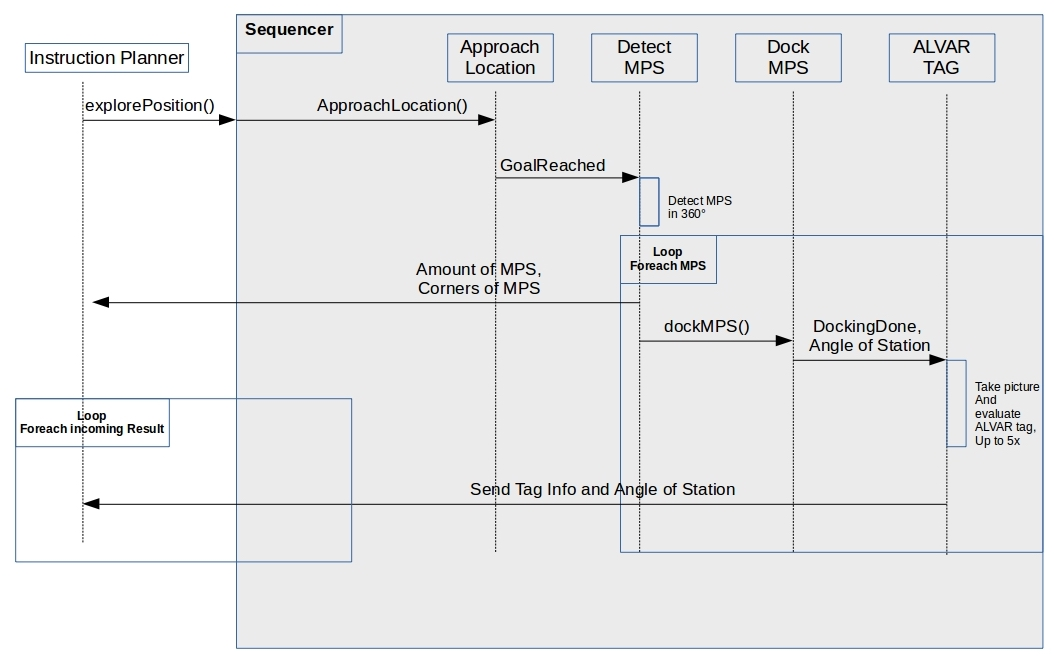
\includegraphics[scale=0.5]{pic/sequenceSequencer.jpg}
\caption{Sequence of the implemented Exploration Phase in the Sequencer}
\label{fig:sequ_overview}
\end{figure}


\subsubsection{Procedure of the Exploration Phase}

The sequence of actions and the calling or triggering of the skill components are implemented in .lisp files.

\begin{itemize}

\item ExplorePosition

The InstructionPlanner starts the Exploration Phase in the Sequencer by calling the \textit{explorePosition()} method. This is the entry point for the sequence of actions for the Exploration Phase. The robot will drive to a predefined position on the field, which is managed by the InstructionPlanner.  

\item Detect MPS

After reaching the position, the robot will perform the detection of the MPS stations. The sequencer triggers the component SmartRobotinoDetection.
Each detected MPS station is sent back to the Sequencer, which manages a list of the detected MPS stations. 
The Sequencer sends the amount of detected MPS stations back to the InstructionPlanner. This is necessary, because the IP needs to know, for how much results he is waiting for, before a new \textit{explorePosition()} command is sent.
For every detected MPS, the Sequencer triggers the SmartMPSRobotinoDocking component.

\item Dock MPS

The SmartMPSRobotinoDocking component tries to dock to the appropriate machine. 
The Docking component gives feedback, whether the docking was successful or not. By telling the Sequencer \textit{Docking done (e.g. success)}, the Alvar Tag Detection component is triggered. This triggering message holds also the angle of the machine, which was calculated in the docking component.

\item ALVAR Tag Detection

The last part of the chain is the ALVAR Tag Detection. It provides an ALVAR Tag, or an error message. 
If an ALVAR Tag gets detected, the Sequencer sends back the angle of the station (from the docking component) and the ALVAR Tag information to the Instruction Planner.

\end{itemize}

\subsubsection{Conclusion }

By implementing the Exploration Phase ( and also the Production Phase later on) in the Sequencing Layer, the big disadvantage of the Instruction Planner design of the former team is solved. The Instruction Planner of 2017 tried to absorb the functionality of the Sequencer of Smartsoft, by implementing a state machine, which represented the Exploration Phase (VERWEIS 2017 REPORT ODER KAPITEL INSTRUCTION PLANNER).
Unfortunately there was not enough time for the team 2018 to implement also the Production Phase in the Sequencer.


